\documentclass[10pt]{article}
\usepackage{titlesec}
\usepackage{geometry}
\geometry{verbose,tmargin=.9in,bmargin=.9in,lmargin=1.0in,rmargin=1.0in}
\usepackage{amsmath,amsfonts,amsthm,amssymb}
\usepackage{url}
\usepackage{color}
\usepackage[usenames,dvipsnames,svgnames,table]{xcolor}
\usepackage[colorlinks=true, linkcolor=red, urlcolor=blue, citecolor=gray]{hyperref}
\usepackage{float}
\usepackage{caption}
\usepackage{subcaption}
\usepackage{graphicx}
\usepackage{wrapfig}
\usepackage{booktabs}
\usepackage{longtable}
\usepackage{enumitem}
\usepackage{multicol}
\usepackage{etoolbox}

\DeclareMathOperator*{\argmin}{arg\,min}
\DeclareMathOperator*{\argmax}{arg\,max}

\definecolor{nyuDarkPurple}{HTML}{330662}
\definecolor{nyuOfficialPurple}{HTML}{57068c}

\newcommand{\spara}[1]{\vspace{.5em}\noindent {\large\sffamily\textcolor{nyuOfficialPurple}{#1}}}
\titleformat{\section}[hang]{\Large\sffamily\color{nyuDarkPurple}}{\thesection}{1em}{}
\titleformat{\subsection}[hang]{\large\sffamily\color{nyuDarkPurple}}{\thesection}{1em}{}
\titleformat{\subsubsection}[hang]{\normalsize\sffamily\color{gray}}{\thesection}{1em}{}

\usepackage{fancyhdr}
\pagestyle{fancy}
\lhead{
\includegraphics[width=4cm]{tandon_long_color.eps}}
\rhead{\thepage}
\pagenumbering{gobble}

\setcounter{secnumdepth}{0}

% math commands
\DeclareMathOperator{\R}{\mathbb{R}}
\newcommand{\E}{\mathbb{E}}

\begin{document}
	
\begin{center}
	\normalsize
	New York University Tandon School of Engineering
	
	Computer Science and Engineering
	\medskip
	
	\large
	CS-UY 4563: Midterm Exam 1. 
	
	Monday, Mar. 9th, 2020, 9:00 - 10:15pm
	
	50 Total Points
	\medskip
\end{center} 

\subsection{Directions}
\begin{itemize}
	\item Show all of your work to receive full (and partial) credit.
	\item If more space is required, you may use extra sheets of paper clearly marked with your name, netid, and the problem you are working on.
\end{itemize}

\subsection{1. Always, Sometimes, Never. (\textbf{\small 12pts -- 3pts each})} 
Indicate whether each of the following statements is ALWAYS true, SOMETIMES true, or NEVER true. \textbf{No justification is necessary to receive full credit for a correct answer}. To earn partial credit if you are wrong, you may provide a short justification or example to explain your choice.
\begin{enumerate}[label=(\alph*)]
	\item The empirical risk of a model is lower than the population risk.
	
	ALWAYS\hspace{1em} \textbf{SOMETIMES}\hspace{1em} NEVER
	
	\color{blue}
	Empirical risk is a random quantity which depends on the data. Even when it's equal to the population risk in expectation, it could be larger or smaller depending on chance.
	\color{black}
	\vspace{1em}
	
	\item You train a multiple linear regression model with varying levels of $\ell_2$ regularization. Let $\vec{\beta}^{(1)} = \argmin_{\vec{\beta}}  \|X\vec{\beta} - \vec{y}\|_2^2 + \lambda_1 \|\vec{\beta}\|_2^2$ and let $\vec{\beta}^{(2)} = \argmin_{\vec{\beta}}  \|X\vec{\beta} - \vec{y}\|_2^2 + \lambda_2 \|\vec{\beta}\|_2^2$. 
	
	If $\lambda_1 > \lambda_2$, is $\|X\vec{\beta}^{(1)}  - \vec{y}\|_2^2 < \|X\vec{\beta}^{(2)}  - \vec{y}\|_2^2$?

	ALWAYS\hspace{1em} SOMETIMES\hspace{1em} \textbf{NEVER}
	
	\color{blue}
%	Since $\lambda_1 > \lambda_2$ we can write $\argmin_{\vec{\beta}}  \|X\vec{\beta} - \vec{y}\|_2^2 + \lambda_1 \|\vec{\beta}\|_2^2 = \argmin_{\vec{\beta}}  \|X\vec{\beta} - \vec{y}\|_2^2 + \lambda_2 \|\vec{\beta}\|_2^2 + \lambda' \|\vec{\beta}\|_2^2$ where $\lambda' = \lambda_1 - \lambda_2$ is positive. 
	By the optimality of $\vec{\beta}^{(1)}$ we have that $\|X\vec{\beta}^{(1)} - \vec{y}\|_2^2 + \lambda_1 \|\vec{\beta}^{(1)}\|_2^2 \leq \|X\vec{\beta}^{(2)} - \vec{y}\|_2^2 + \lambda_1 \|\vec{\beta}^{(2)}\|_2^2$. At the same time, By the optimality of $\vec{\beta}^{(b)}$, we have that  $\|X\vec{\beta}^{(2)} - \vec{y}\|_2^2 + \lambda_2 \|\vec{\beta}^{(2)}\|_2^2 \leq \|X\vec{\beta}^{(1)} - \vec{y}\|_2^2 + \lambda_2 \|\vec{\beta}^{(1)}\|_2^2$. Negating this inequality gives $-\|X\vec{\beta}^{(1)} - \vec{y}\|_2^2 - \lambda_2 \|\vec{\beta}^{(1)}\|_2^2 \leq -\|X\vec{\beta}^{(2)} - \vec{y}\|_2^2 - \lambda_2 \|\vec{\beta}^{(2)}\|_2^2$. Adding the two inequalities gives $(\lambda_1-\lambda_2) \|\vec{\beta}^{(1)}\|_2^2 \leq (\lambda_1-\lambda_2)  \|\vec{\beta}^{(2)}\|_2^2$, which means that $ \|\vec{\beta}^{(1)}\|_2^2 \leq  \|\vec{\beta}^{(2)}\|_2^2$ since $(\lambda_1 - \lambda_2)$ is positive.
	
	But as we already noted, we also have that $\|X\vec{\beta}^{(2)} - \vec{y}\|_2^2 + \lambda_2 \|\vec{\beta}^{(2)}\|_2^2 \leq \|X\vec{\beta}^{(1)} - \vec{y}\|_2^2 + \lambda_2 \|\vec{\beta}^{(1)}\|_2^2$. If $ \|\vec{\beta}^{(1)}\|_2^2 \leq  \|\vec{\beta}^{(2)}\|_2^2$, this can only be true if $\|X\vec{\beta}^{(2)}  - \vec{y}\|_2^2 \leq \|X\vec{\beta}^{(1)}  - \vec{y}\|_2^2$.
	\color{black}
	\vspace{1em}
	
	
	
	\item The linear classifier found by logistic regression minimizes error rate ( $0$-$1$ loss)  on the training data. 
	
	ALWAYS\hspace{1em} \textbf{SOMETIMES}\hspace{1em} NEVER
		
	\color{blue}
	In general it does not, unless we get lucky. It minimizes the logistic loss. An answer of NEVER would also be accepted.
	\color{black}
	\vspace{1em}
	
%	\item For convex functions $f(x)$ and $g(x)$, $f(x)\cdot g(x)$ is convex.
%	
%	ALWAYS\hspace{1em} SOMETIMES\hspace{1em} NEVER\vspace{4em}
	
	\item Consider a multiple linear regression problem where each data example has the form $(\vec{x},y) = ([x_1,x_2],y)$. Transform the predictor variables by adding quadratic terms, so each new data example has the form $(\vec{x}_{trans},y)= ([x_1,x_2,x_1^2, x_2^2, x_1x_2],y)$. Let $L^*$ be the minimum training loss for the original problem and let ${L}_{trans}^*$ be the minimum training loss for the transformed problem. Is ${L}_{trans}^* \leq L^*$?
	
	\textbf{ALWAYS}\hspace{1em} SOMETIMES\hspace{1em} NEVER
	
	\color{blue}
	For any $\vec{\beta} = [\beta_1,\beta_2]$, $L_{trans}([\beta_1,\beta_2, 0,0,0]) = L([\beta_1,\beta_2])$. So it is always possible to find parameters that ensure $L_{trans} \leq L$. It must therefore be that $\min L_{trans} \leq \min L$. 
	\color{black}
	\vspace{1em}
	
	

\end{enumerate}

\subsection{2. Model Diagnosis Short Answer (\textbf{\small 8pts})}
You are trying to solve a prediction problem using a multiple linear regression model with $\ell_2$ loss. 
You first split the data set into a train set (80\%) and a test set (20\%). You then train the model on the train set to obtain a parameter vector $\vec{\beta}$. Using $\vec{\beta}$, you evaluate the average squared loss of the regression model on the train and test set, separately.


For each of the following scenarios, circle all answers that apply.  \textbf{No justification is necessary to receive full credit for a correct answer}. To earn partial credit if you are wrong, you may provide a short justification.
\begin{enumerate}[label=(\alph*)]
	\item  (4pts) The average squared loss on the train set is $1.5$ and the average squared loss on the test set is $12.6$. \textbf{Which of the following techniques is likely to improve your average test loss?} 
	
	\vspace{1em}\textbf{REGULARIZATION}\hspace{.25em} \textbf{FEATURE SELECTION}\hspace{.25em} FEATURE TRANSFORM \hspace{.25em} DATA SCALING
	
	\vspace{1em}
	\color{blue}
	We appear to be overfitting since our train loss is much less than our test loss. Regularization or feature selection would be the most appropriate cures. Feature transformation typically leads to a richer model, so only makes overfitting worse. And data scaling doesn't do anything for linear regression! 
	\color{black}
	\vspace{1em}

	
	\item (4pts) The average squared loss on the train set is $10.2$ and the average squared loss on the test set is $9.9$. \textbf{Which of the following techniques is likely to improve your average test loss?}
	
	\vspace{1em}REGULARIZATION\hspace{.25em} {FEATURE SELECTION}\hspace{.25em} \textbf{FEATURE TRANSFORM} \hspace{.25em} DATA SCALING
	
	\vspace{1em}
	\color{blue}
	We appear to be performing poorly on both train and test loss, so we might need a richer model. The best cure would therefore be some sort of feature transformation. Of course, it's not guaranteed to work, but would be worth a try.
	\color{black}
	\vspace{1em}
	
	

\end{enumerate}




\newpage
\subsection{3. Model Diagnosis 2 (\textbf{\small 10pts})}
Consider the following scatter plots of data for three binary classification problems. $x_1$ and $x_2$ are the independent variables and class labels are indicated by points with a different shape and shade.

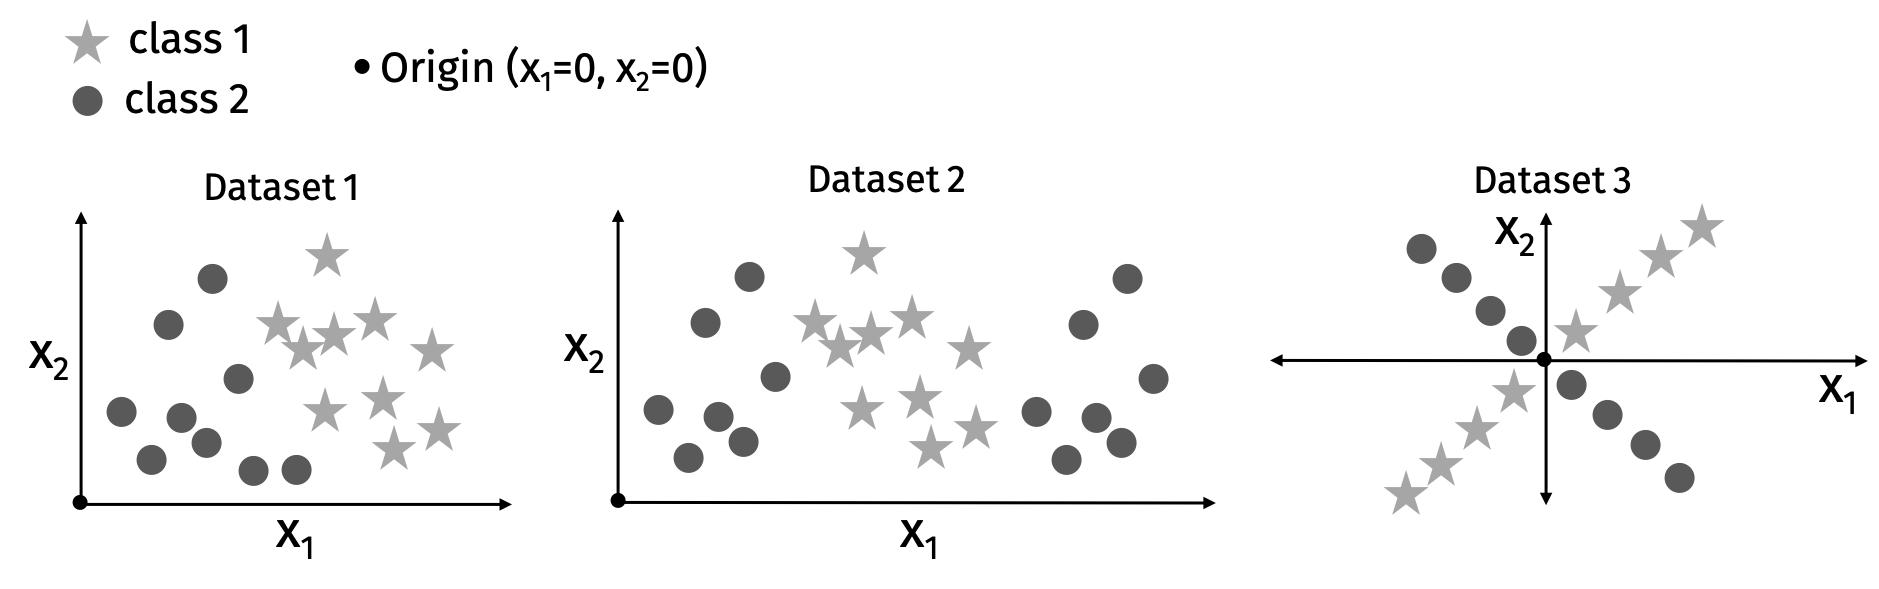
\includegraphics[width=\textwidth]{examp_datasets.png}



\begin{enumerate}[label=(\alph*)]
	\item (4pts) Indicate which of the three clustering problems could be solved to high accuracy (small error rate) using a logistic regression model with no regularization and no feature transformations. 
	
	\vspace{1em}
	\color{blue}
	Logistic regression will perform well on any dataset which can be classified using a \emph{linear classifier}. This would include \textbf{only Dataset 1}. Logistic regression will perform poorly on Datasets 2 and 3.
	\color{black}
	\vspace{1em}
	
	\item (6pts) For any of the problems that you believe are not \emph{directly solvable} with logistic regression, suggest a possible feature transformation which \emph{would make it possible} to obtain a high accuracy solution with logistic regression. For each problem, your solution should be a set of new features $\phi_1(x_1,x_2), \phi_2(x_1,x_2), \ldots, \phi_q(x_1,x_2)$ that depend on the original features $x_1$ and $x_2$. You may use as large a $q$ as you need.
	
	\vspace{1em}
	\color{blue}
	There are many possible answers here:
	\begin{description}
		\item[Dataset 2] $\phi_1= x_1, \phi_2= x_2, \phi_3 = x_1^2, \phi_4 = x_2^2, \phi_5 = 1$ would work since it would allow use to classify using a shifted oval: e.g. classify star if $(x_1 - 2)^2 + .8(x_2 - 1)^2 < .5$. 
		\item[Dataset 3] $\phi_1 = x_1/x_2$ works. For Class 1 this is always $\approx 1$ and for Class 2 it is $\approx -1$, so these values can be seperated via a linear classifier. 
		
	\end{description}
	\color{black}
	\vspace{1em}


\end{enumerate}


\vspace{10em}

\newpage
\subsection{4. Loss Minimization. (\textbf{\small 10pts})}

For data with one predictor and one target: $(x_1, y_1), \ldots, (x_n, y_n)$, consider a linear regression model:

\begin{align*}
f_{\beta_0,\beta_1}(x) = \beta_0 + \beta_1 x
\end{align*}
with \emph{exponential loss}:
\begin{align*}
L(\beta_0,\beta_1) = \sum_{i=1}^n e^{(y_i - f_{\beta_0,\beta_1}(x_i))^2}
\end{align*}

\begin{enumerate}[label=(\alph*)]
	\item (5pts) Write down an expression for the gradient of the loss $L$.
	
	\vspace{1em}
	\color{blue}
	We can compute both partial derivatives to get the gradient. For both we need to use chain rule:
	\begin{align*}
	\frac{\partial L}{\partial \beta_0} =\sum_{i=1}^n -2\cdot (y_i - \beta_0 - \beta_1 x_i)\cdot e^{(y_i - \beta_0 - \beta_1 x_i)^2}
	\end{align*}
	\begin{align*}
	\frac{\partial L}{\partial \beta_1} = \sum_{i=1}^n -2x_i\cdot (y_i - \beta_0 - \beta_1 x_i)\cdot e^{(y_i - \beta_0 - \beta_1 x_i)^2}
	\end{align*}
	And then we have $\nabla L(\beta_0, \beta_1) = \begin{bmatrix}\partial L/\partial \beta_0 \\ \partial L/\partial \beta_1 \\\end{bmatrix}$.
	
	If you wanted to do everything in matrix form, let $\mathbf{X}$ be a data matrix with first column containing $x_1, \ldots, x_n$ and second column containing all $1$s. Then let $\vec{w} = (\vec{y}-\mathbf{X}\vec{\beta})\cdot exp(\vec{y}-\mathbf{X}\vec{\beta})$ where all operations are applied entrywise. Then the gradient is $\textbf{X}^T \vec{w}$.
	\color{black}
	\vspace{1em}
	
	\item (2pts) Name two algorithms/methods which could be used to minimize $L$.
		\vspace{1em}
	\color{blue}
		\begin{itemize}
			\item Brute force search. 
			\item Gradient descent. 
		\end{itemize}
	\color{black}
	
	\item (3pts) In general, is this exponential loss more or less robust to outliers when compared to $\ell_2$ loss? How about when compared to $\ell_\infty$ loss? 
	
	\vspace{1em}
	\color{blue}
	If the linear model under exponential loss is effected \emph{more} by an outlier, we say the loss is \emph{less} robust.
	
	It is therefore less robust than $\ell_2$ loss because the loss function punishes outliers significantly more: you pay a cost of $e^{\text{squared error}}$ instead of just the square error. It will thus try to more closely fit outliers.
	On the other hand, the exponential loss is more robust than $\ell_\infty$ loss, which punishes outliers pretty much as much as possible: we only care about the loss of the worst data example.
	\color{black}
	\vspace{1em}
\end{enumerate}


\newpage

\subsection{5. Bayesian Crab Classification (\textbf{\small 10pts})}
A biologist is collecting specimens from two species of crabs, species $S_0$ and $S_1$. These species live in the same habitat and look similar to the human eye. To accelerate crab sorting by species, the biologist wants to develop a simple classification rule based on body measurements. She observes that the ratio of \emph{forehead breadth} to overall \emph{body length} differs between crabs in species $S_0$ and $S_1$. The biologist proposes to measure this ratio (denoted by $R$) and use it as a single predictor variable for classification.

The biologist assumes that the crab data comes from a ``mixture of Gaussians'' probabilistic model. In particular, she assumes that for each species, $R$ follows a normal (Gaussian) probability distribution, with different parameters for each species. The biologist makes the following concrete observations:
\begin{itemize}
	\item $35\%$ of all crabs collected belong to $S_0$ and the remaining $65\%$ belong to $S_1$. 
	\item For crabs in $S_0$, the average value of $R$ is $.5$. For crabs in $S_1$, the average value of $R$ is $.4$. 
	\item For both species, the standard deviation of $R$ is $.1$.
\end{itemize}


\begin{enumerate}[label=(\alph*)]
	\item (6pts) Suppose we collect a new crab with forehead breadth to body length ratio $R_{new}$.  The biologist would like to assign this crab to $S_0$ or $S_1$ using a maximum a posterior (MAP) classification rule. Denote this rule by $f: \R\rightarrow \{S_0,S_1\}$. The rule takes as input the ratio $R_{new}$ and outputs $S_0$ or $S_1$.

	Write down all mathematical expressions that would need to be evaluated to compute $f$ for a given input $R_{new}$. Your expressions do not need to be simplified, but they should not involve unknown variables besides $R_{new}$. \textbf{Hint:} Use Bayes rule.
	

	
	\vspace{1em}
	\color{blue}
	To implement a MAP estimator we need to compute:
	\begin{align*}
	&\Pr(S_0 \mid R_{new}) & &\text{and} & &\Pr(S_1 \mid R_{new})
	\end{align*}
	Using Bayes rule we have:
	\begin{align*}
	\Pr(S_0 \mid R_{new}) & = \frac{\Pr(R_{new}\mid S_0)\Pr(S_0)}{\Pr(R_{new})} & &\text{and} & \Pr(S_1 \mid R_{new}) & = \frac{\Pr(R_{new}\mid S_1)\Pr(S_1)}{\Pr(R_{new})}
	\end{align*}
	Note that, we have:
	\begin{align*}
	\Pr(S_0) &=  .35 & &\text{and} & \Pr(S_1) &=  .65.
	\end{align*}
	And using the equation for the Gaussian distribution, we also have:
	\begin{align*}
	\Pr(R_{new}\mid S_0) &=  \frac{1}{\sqrt{2\pi}\cdot .1}e^{-\frac{(R_{new} - .5)^2}{2\cdot .1^2}} & &\text{and} & \Pr(R_{new}\mid S_1) &=  \frac{1}{\sqrt{2\pi}\cdot .1}e^{-\frac{(R_{new} - .4)^2}{2\cdot .1^2}}.
	\end{align*}
	\color{black}
	\vspace{1em}
	
	\item (4pts) Show that, for this problem, the classification rule $f$ has the following form:
	\begin{align*}
	f(R_{new}) = \begin{cases}
	S_0 \text{ if } R_{new} \geq \lambda \\
	S_1 \text{ if } R_{new} < \lambda,
	\end{cases}
	\end{align*}
	for some fixed threshold parameter $\lambda$ (you do not need to explicitly compute $\lambda$).
	
	\color{blue}
	\textbf{Note:} A less formal argument than what I give below would suffice.
	
	
	The MAP classification rule $f$ is as follows:	
	\begin{align*}
	f(R_{new}) = \begin{cases}
	S_0 \text{ if } \Pr(S_0 \mid R_{new}) \geq \Pr(S_1 \mid R_{new}), \\
	S_1 \text{ if } \Pr(S_0 \mid R_{new}) < \Pr(S_1 \mid R_{new}).
	\end{cases}
	\end{align*}
	Substituting in our equations from part (a), we see that we will classify a crab with ratio $R_{new}$ into class $S_0$ under this rule if:
	\begin{align*}
	f(R_{new}) &= S_0 \text{ if} & &\frac{.35\frac{1}{\sqrt{2\pi}\cdot .1}e^{-\frac{(R_{new} - .5)^2}{.02}}}{\Pr(R_{new})} \geq \frac{.65\frac{1}{\sqrt{2\pi}\cdot .1}e^{-\frac{(R_{new} - .4)^2}{.02}}}{\Pr(R_{new})}
	\end{align*}
	which is equivalent to checking if
	\begin{align*}
	\label{eq:check}
	f(R_{new}) &= S_0 \text{ if} & &.35 e^{-\frac{(R_{new} - .5)^2}{.02}} \geq .65e^{-\frac{(R_{new} - .4)^2}{.02}}. 
	\end{align*}
	Taking logs and rearranging, this in turn is equivalent to checking:
	\begin{align*}
		f(R_{new}) &= S_0 \text{ if} & & (R_{new} - .4)^2 - (R_{new} - .5)^2 \geq .02\log(.65) - .02\log(.35) \\
		f(R_{new}) &= S_0 \text{ if} & &.2\cdot R_{new} \geq .02\log(.65) - .02\log(.35) - .16 + .25
	\end{align*}
	So clearly we classify in $S_0$ if $R_{new} \geq \lambda$ for some $\lambda$.
	
	\color{black}
		
	\item (3pts -- extra credit) Given the biologist's data above, will the threshold $\lambda$ for the MAP classification rule be EQUAL TO, LARGER, or SMALLER than $.45$? Justify your answer in a sentence or two. This problem can be solved without a calculator. 
	
	\color{blue}
	$\lambda$ will be \textbf{LARGER} than $.45$. It would equal .45 exactly if $\Pr(S_0) = \Pr(S_1) = .5$. However, since the prior probability of $\Pr(S_1)$ is larger, we will classify an example as $S_1$ even if its ratio slightly exceeds $.45$. To see this from the calculations above, note that $(- .16 + .25)/.2 = .45$ and $\log(.65) - \log(.35)$ is positive. So $\lambda > .45$. The actually threshold would be around $.512$. 
	\color{black}
	
\end{enumerate}

\end{document}